% !TEX root = main.tex

\section{Результаты расчётов}

\begin{align*}
    \hat{\mu} &= 14.35\\
    S^{2} &= 1.28\\
    (\underline{\mu},\;\overline{\mu}) &= (14.29,\;14.85)\\
    (\underline{\sigma^{2}},\;\overline{\sigma^{2}}) &= (0.79,\;1.67)
\end{align*}


\section{Графики}

$y=\hat{\mu}(\vec{x}_{N}),\; y=\hat{\mu}(\vec{x}_{n}),\; y=\underline{\mu}(\vec{x}_{n}),\; y=\overline{\mu}(\vec{x}_{n})$ как функций объема $n$ выборки, где  $n$ изменяется от $1$ до $N$.

\begin{figure}[h]
    \centering
    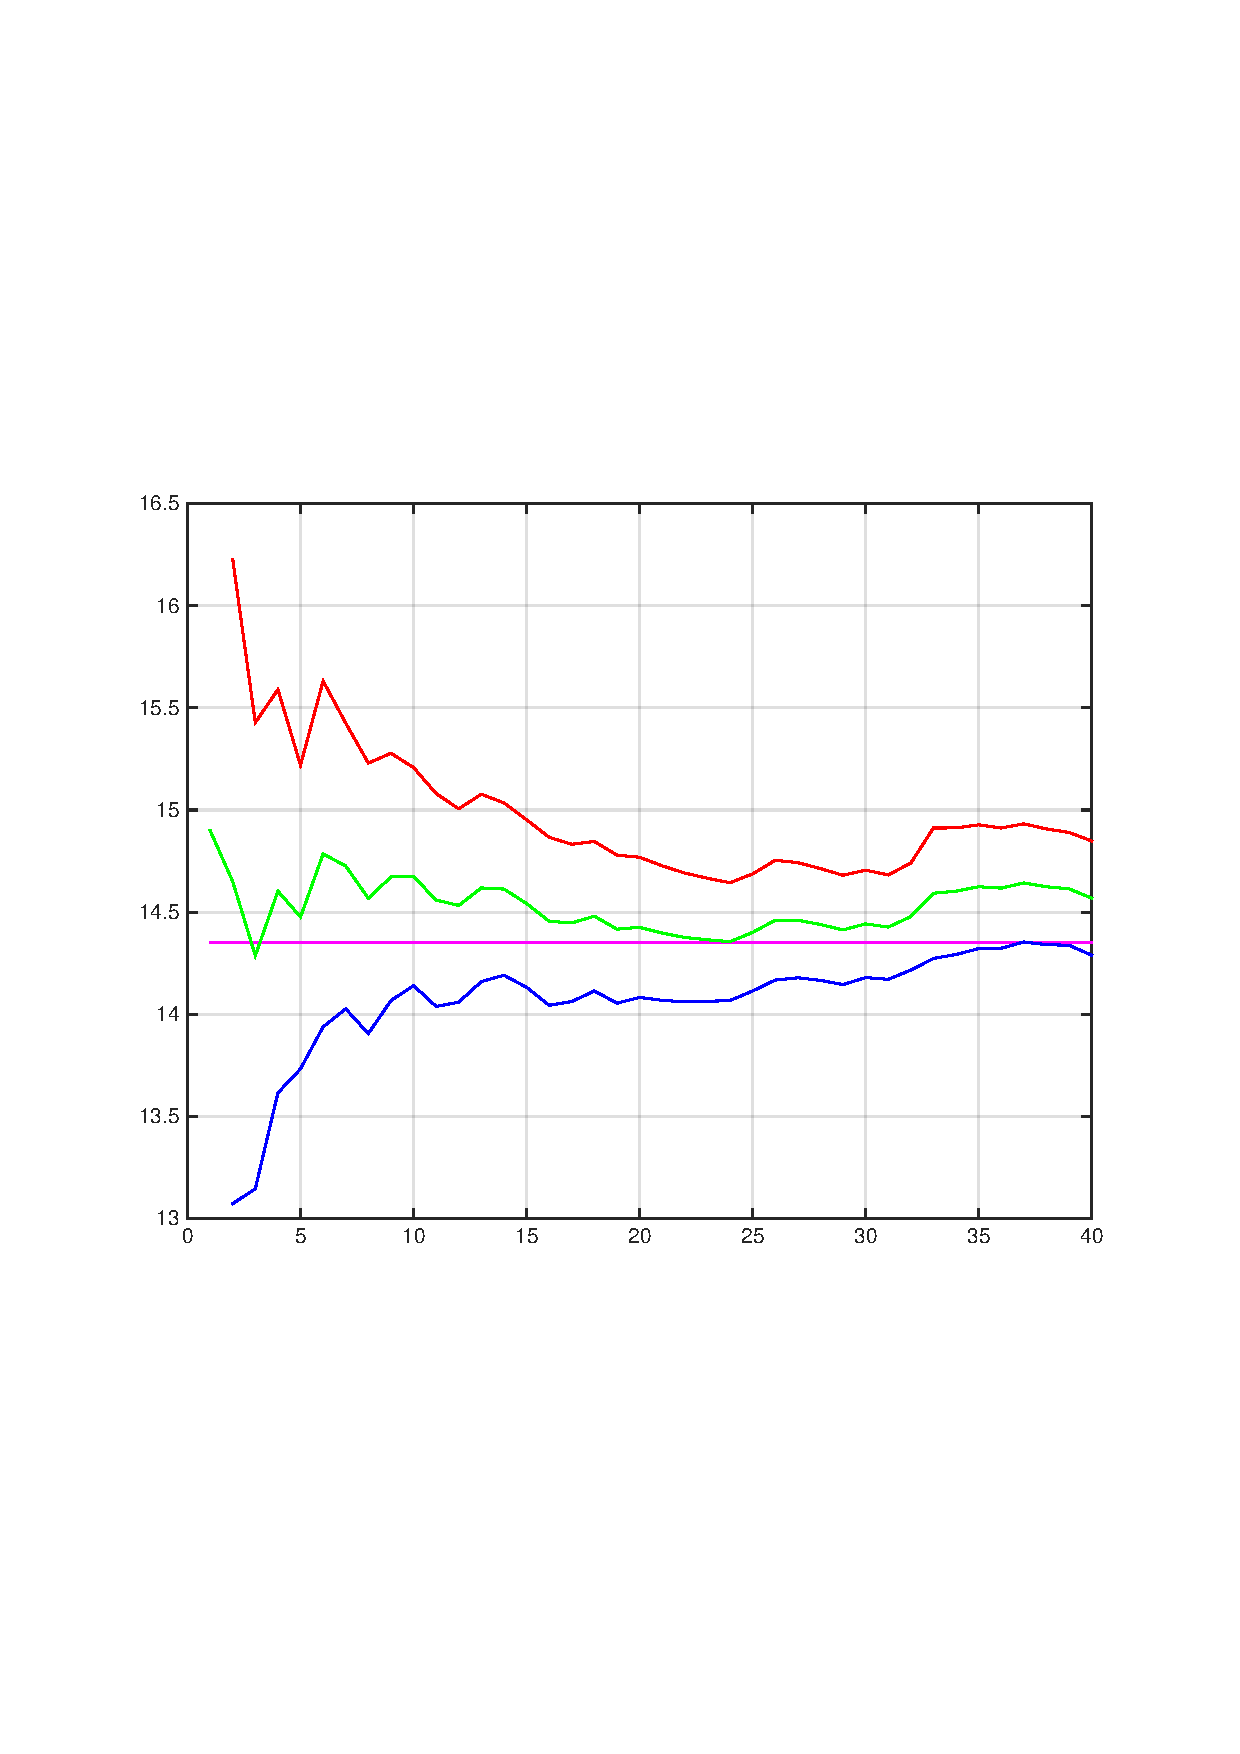
\includegraphics[width=0.7\textwidth]{graphs/figure1.pdf}
\end{figure}



\newpage

$y=S^{2}(\vec{x}_{N}),\; y=S^{2}(\vec{x}_{n}),\; y=\underline{\sigma^{2}}(\vec{x}_{n}),\; y=\overline{\sigma^{2}}(\vec{x}_{n})$ как функций объема $n$ выборки, где $n$ изменяется от $1$ до $N$.

\begin{figure}[h]
    \centering
    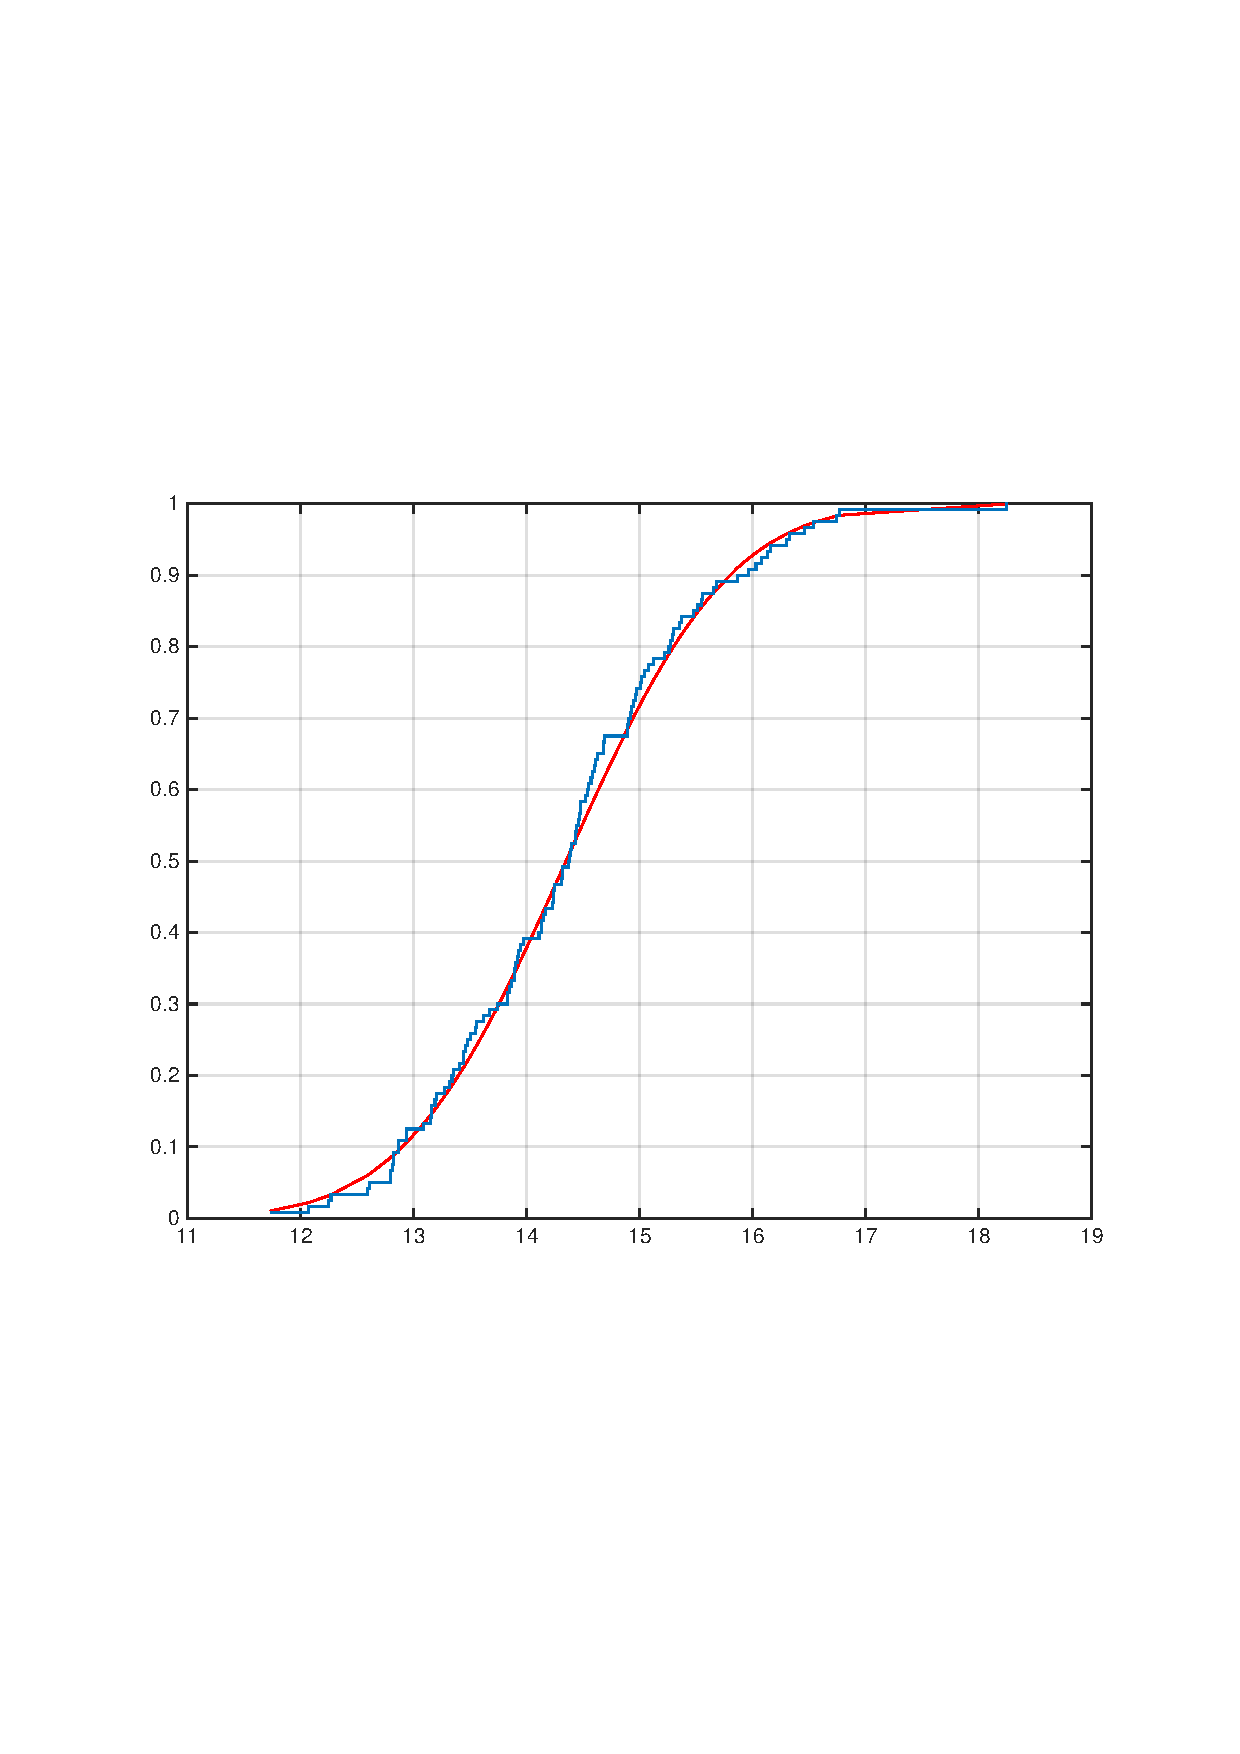
\includegraphics[width=0.7\textwidth]{graphs/figure2.pdf}
\end{figure}